\section{Experiments}
\label{sec:intro}

We conducted three different experiments where we evaluated the accuracy of the models in terms of how many test commands were exactly translated
into corresponding test actions. 
\citet{Lake:Baroni:2017} found that RNNs models are achieve nearly perfect performance when tested on a random split of SCAN but accuracy drops significantly
(down to around 20\% for their best performing model) when the network is tested on composing new meanings after being exposed only to shorter samples.

In order to make our results comparable with previous work on SCAN each training set consists of 100,000 examples sampled with replacement
from each related train/test split. We decided to replicate experiment 1 of \cite{Lake:Baroni:2017} that simply uses a random split
of the SCAN dataset divided into a train (80\%) and test (20\%) set. This would act as a first comparison with the RNNs results reported in their work.

\subsection{Experiment 1: random split and primitive generalization}
\label{subsec:exp1}

After a preliminary experiment we found a subset of parameters showing reasonable performance and conduceted a large hyperparameters
search on every split.
We varied batch sizes (in term of number of tokens in the batch: 25, 50, 100, 200, 500 and 100), learning rates
0.1, 0.01, 0.001), the embedding dimensions (128, 256, 512), amount of dropout used (0, 0.25, 0.5) \cite{srivastava:eta:2014}, number of convolutional
layers for both the encoder and decoder (6, 7, 8, 9, 10) and width of the convolutional kernel (3, 4, 5).
We then cross validated the top-300 models across 5 different runs. Accuracy and standard deviation are presented in figure \ref{fig:exp1}. 
We inspected the average accuracy of the model note that the amount of standard deviation of the top-300 models reached a performance range with a lower limit that was always
considerably lower than the best model for each split, making us think that considering the top-300 models was
a right choice that included tha real best model for every split. In other words, the accuracy for the best model and the 300th one formed a large range.
\footnote{This might not seem the case for the results on the random split where the range is (95.17, 99.97). However the standard deviation across all 300 models does not
exceed 2.7}
When analyzing the the resulting models for every split we computed a \textbf{best overall model} across all splits which
was a model trained with a learning rate of 0.01, a 25 tokens per batch, dropout applied with probability 0.25, it had 6 layers in both the encoder and the decoder,
embedding dimension of 512, a convolutional kernel of width 5. Such model was ranked 13th on the random split (with an accuracy of 99.92\% off by 0.05\%), 
32th on the jump split (60.67\% accuracy, off by 8.62\% compared to the top performing model for the split),
and 2nd in the template split (53.25\% accuracy, off by 3.45\%)
Experiment 2 and 3 in section \ref{subsec:exp2} and \ref{subsec:exp3} used the aforementioned model.

\begin{figure}[h]
    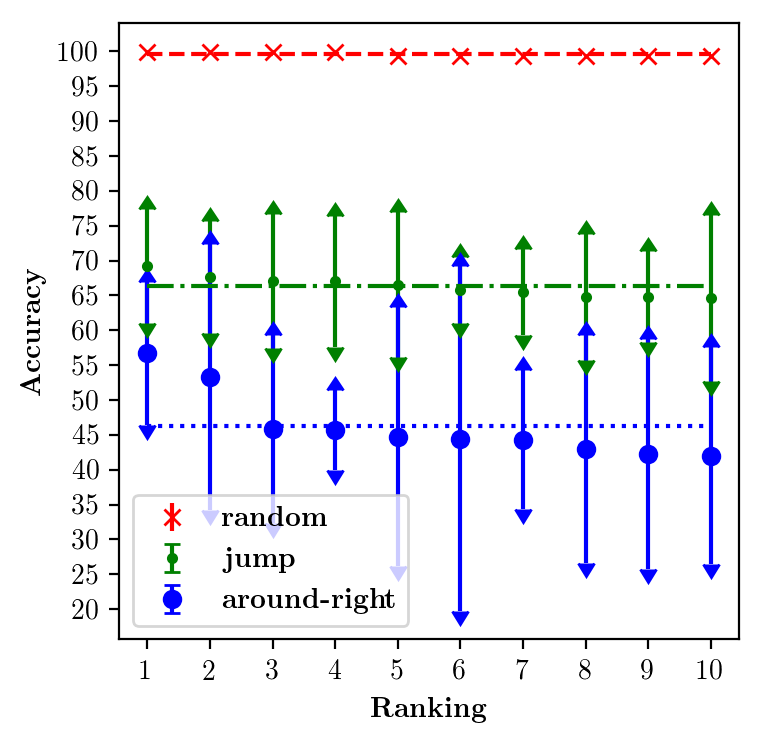
\includegraphics[width=.5\textwidth,keepaspectratio]{figures/accuracies_all_splits.png}
    \centering
    \caption{Accuracies for the top-10 models on every split. Dashed lines report split means}
    \label{fig:exp1}
\end{figure}


% 219.08612pt
% 3.0314
\subsection{Experiment 2: second-order modifiers and kernel study}
\label{subsec:exp2}

\iffalse

\begin{figure}[h]
    \centering
    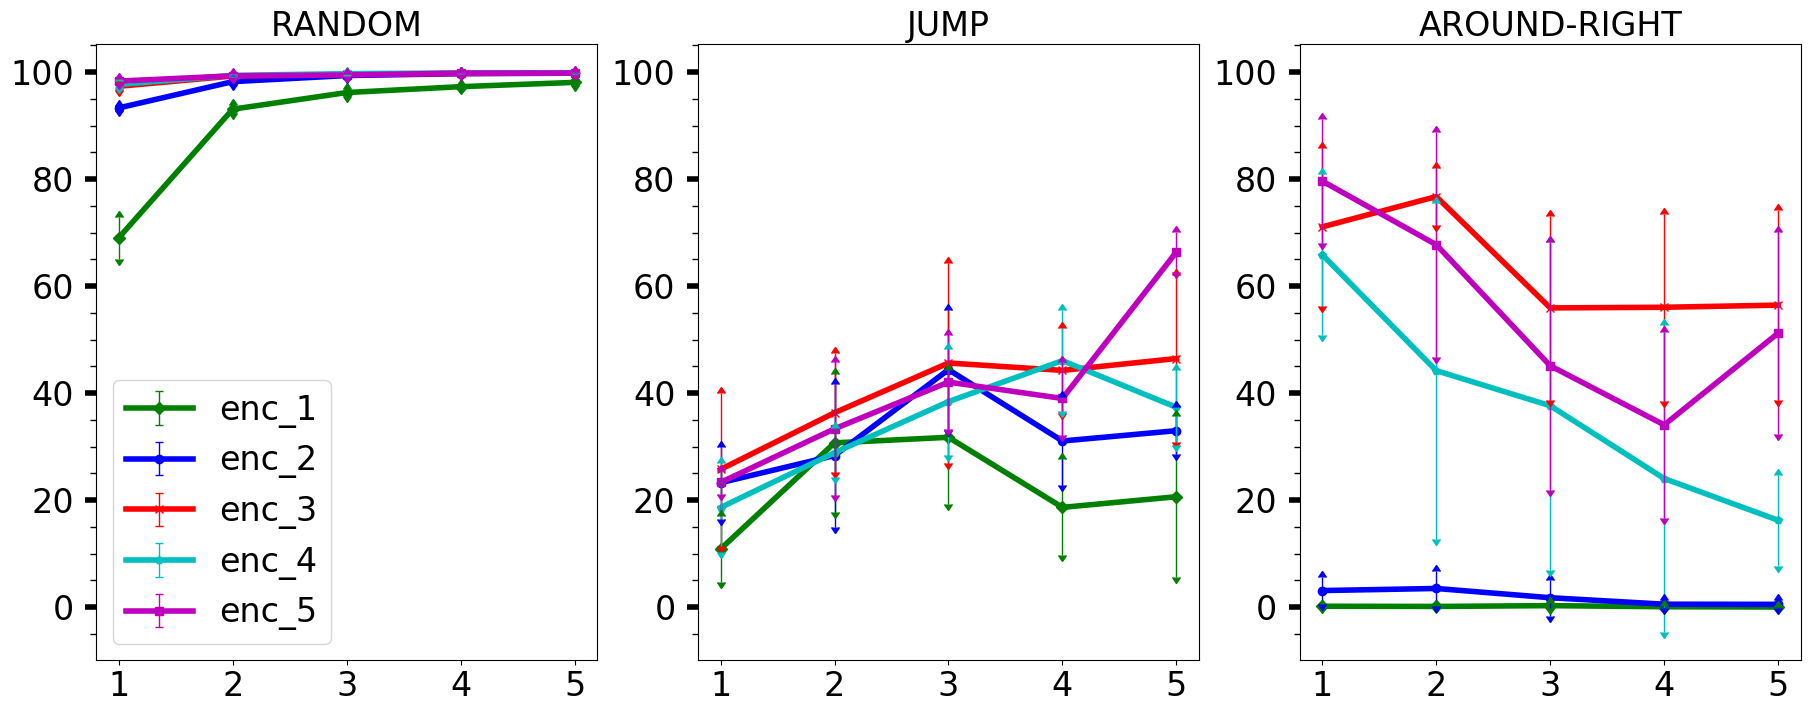
\includegraphics[width=.5\textwidth,keepaspectratio]{figures/kernel_exp.png}
    \caption{Accuracy for kernel experiment}
    \label{fig:kernel_exp}
\end{figure}

\fi

\subsection{Experiment 3: ablation study on attention}
\label{subsec:exp3}

Due to the importance of the attention mechanism for our convolutional architecture we decided to conduct study with the best-overall model
and the attention only on specific layers. Results are presented in \ref{fig:exp3}...

\begin{figure}[h]
    \centering
    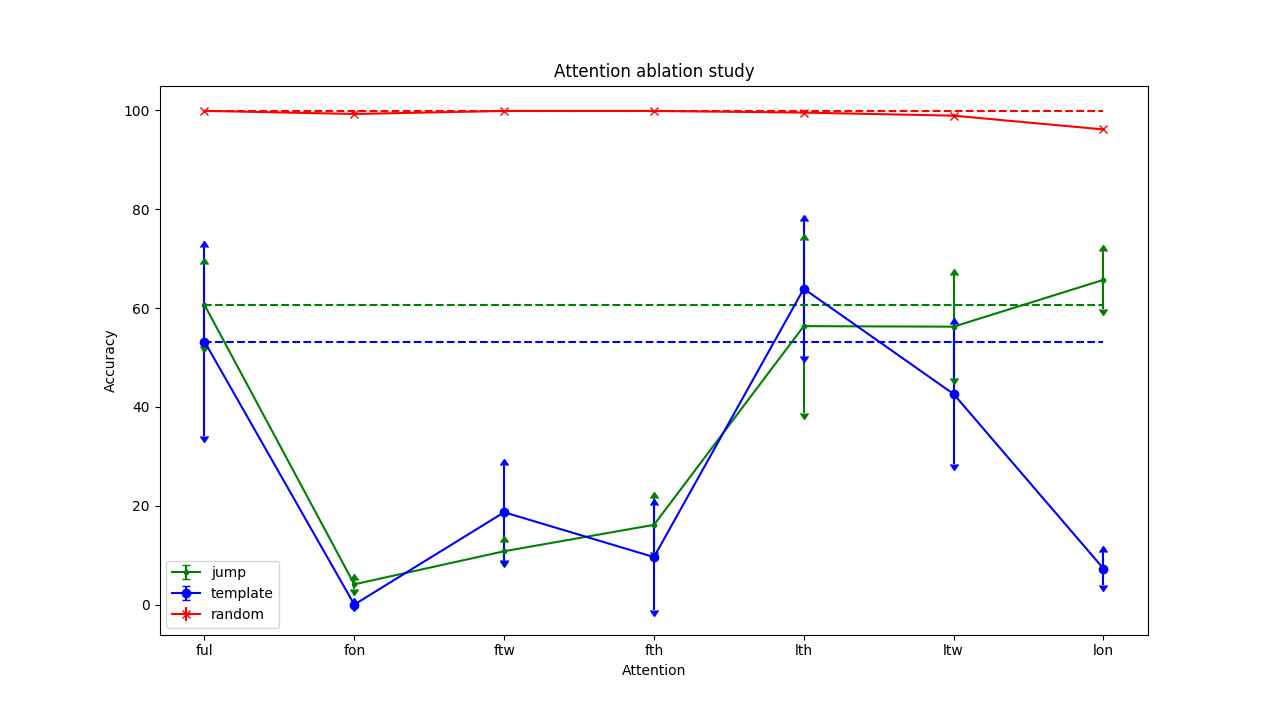
\includegraphics[width=.5\textwidth,keepaspectratio]{figures/attention_exp.png}
    \caption{Accuracy for attention experiment}
    \label{fig:exp3}
\end{figure}

